In clinical PET imaging one of the main clinical and research needs is imaging information over the whole-body. For example most PET oncology applications require whole body coverage to detect and characterise the primary disease and any metastatic disease. This need for whole body coverage is not exclusive to oncology, many clinical and research applications can benefit from this type of information. In this chapter we will describe the main principles behind use of multi-bed PET acquisitions, their extension to dynamic imaging and our work in implementing and optimising dynamic whole body acquisition protocols on the Signa PET/MR system. 

\section{Static WB PET}
The first suggestion and optimization work in extending the effective A-FOV of PET scans using multiple bed positions was by made by Dahlbom \textit{et al.}~\cite{Dahlbom1992}. This work was made on PET systems operated in 2D mode, where a bed displacement of approximately equal to the system A-FOV was used to increase the acquisition effective A-FOV. As systems became capable of acquiring in 3D mode, which offers increased sensitivity but results in axial varying sensitivity profiles, different strategies were needed for multi-bed acquisitions. The two methods suggested and developed are the \textit{Step and Shoot}(SS) and the \textit{Continuous Bed Motion}(CBM) acquisition methods. 

\subsection{Step and Shoot}
The SS method makes use of multiple bed positions that are partially overlapped in the axial direction to increase the sensitivity of the acquisition at the edges of each beds FOV, by combining data of adjacent beds over the overlapping region as shown in figure~\ref{fig3_1:fullOverlap}. One way of combining the multi-bed datasets is to reconstruct each bed individually, displace the reconstructed images according to their axial location and combine them using weighted averaging~\cite{Schubert1996}. This method has prevailed in clinical PET systems that use the SS acquisition method, as it does not require addition considerations in the reconstruction process of each bed and the combination of bed images can be performed post-reconstruction. Alternatively the axial displacement of each bed raw dataset can be performed during the projection and back-projection process in iterative reconstruction, which then directly results in the reconstruction of the whole-body image~\cite{Ross2004}. Use of the overlap data in iterative reconstruction can potentially result to improved noise characteristics at the overlapping regions, as the full sampled statistics over these regions are combined prior to each image update~\cite{Ross2004,Stute2014}. 
%
\begin{figure} [ht!]
\centering
\includegraphics[scale=0.5,angle=0]{3_Results/3_1_DWB_Optimization/figures/SensitivityProfiles_fullOverlap.png}
\caption{Relative axial sensitivity of individual beds (top) and combined sensitivity profile (bottom) for approximately 50\% overlap.} 
%TODO: Add over-scan in the CBM D-WB protocols. 
\label{fig3_1:fullOverlap}
\end{figure}
%
The amount of overlap is a parameter to select according to the needs of the axial sensitivity profile.  The axial sensitivity profile for the Signa PET-MR system is shown in figure~\ref{fig3_1:fullOverlap}, where for a completely uniform axial sensitivity profile an overlap of 44 slices (\~50\% of A-FOV) is required.
The amount of overlap used depends on the needs for uniformity in axial sensitivity and reconstructed image noise. This in term will also depend on the used reconstruction type and the activity distribution of the imaged subject~\cite{Schubert1996}. 
For standard clinical scanning at the Signa PET-MR an overlap of \~27\% is used by default, to balance between sensitivity uniformity and examination time for standard WB examinations. The trade-off is made to accommodate longer effective A-FOV in the same acquisition time or to reduce acquisition time by use of less bed positions to image the same scan length. Examples of three overlapping options and the provided coverage are shown in figure~\ref{fig3_1:decreasingOverlap} and~\ref{fig3_1:BodyCoverage} figure respectively.
Many clinical WB protocols actually require imaging of approximately half the length of the body, from head to thighs, which can be accommodated with 5 or 6 bed positions. When full body coverage is required the number of beds is increased to 9 or 10. In DWB acquisitions where fast scanning is crucial the overlap can be decreased to maintain the same coverage with a lesser number of bed positions, as shown in option(C) of figure~\ref{fig3_1:BodyCoverage}. 
%
\begin{figure} [ht!]
\centering
\includegraphics[scale=0.5,angle=0]{3_Results/3_1_DWB_Optimization/figures/SensitivityProfiles_3Options.png}
\caption{Relative axial sensitivity of 5 bed positions with decreasing overlap.} 
%TODO: Add over-scan in the CBM D-WB protocols. 
\label{fig3_1:decreasingOverlap}
\end{figure}
%
%
\begin{figure} [ht!]
\centering
\includegraphics[scale=0.5,angle=0]{3_Results/3_1_DWB_Optimization/figures/SensitivityProfiles_overHuman.png}
\caption{Combinations of overlap and number of beds for static (A\&B) and dynamic whole-body imaging(C). Relative axial sensitivity is shown in shades of red, with bed start (\protect\tikz[baseline]{\protect\draw[line width=0.5mm] (0,.8ex)--++(1,0) ;}) and end (\protect\tikz[baseline]{\protect\draw[line width=0.5mm,densely dashed] (0,.8ex)--++(1,0) ;}) positions.} 
%TODO: Add over-scan in the CBM D-WB protocols. 
\label{fig3_1:BodyCoverage}
\end{figure}



\subsection{Continuous Bed Motion}
Continuous Bed Motion was proposed as an extension of step and shoot acquisition performed with small steps, to provide uniform axial sensitivity profiles without the need of overlaps~\cite{Dahlbom2001,Brasse2002}. In clinical CBM acquisition protocols prompt data as well as bed positions information are stored in list-mode during the examination, with the data being sorted after or during the examination in sinograms (refereed as "chuncks") before reconstruction. The velocity of the bed movement can be adjusted depending on the amount of desired collected statistics, similar to the acquisition time per bed in step and shoot acquisitions. With recent systems the bed velocity can also be varied within an examination according to the needs and distribution of the imaged activity~\cite{Panin2014}. Beyond the potential technical gains, CBM protocols have also been shown to aid in patient comfort during examination~\cite{Schatka2016}. 

In particular for dynamic whole-body imaging many aspects of CBM acquisition can be beneficial over SS imaging~\cite{Karakatsanis2016}.  

\section{Dynamic WB PET}
As outlined in the Introduction and Methods section, clinical and research applications can benefit from dynamic whole-body (DWB) PET information. In clinical applications DWB data can be used to construct fully quantitative parametric images for diagnosis and response monitoring of disease and pathology over the whole body. In research DWB information can enable studying of the whole body organism and interactions between different tissues, organs or compartments. 

Although recent advancements in PET have led to development of PET/CT systems with increased A-FOV, with approximately half~\cite{Karp2020,Siegel2020} or even total-body axial coverage~\cite{Cherry2018}, the majority of PET systems in use are limited in the range from 15 to 26 cm~\cite{Vandenberghe2020}. 
Based on the same principles and methods used in static WB PET imaging, DWB protocols have been developed with use of repeating whole-body passes (often refereed as "sweeps"). These can be implemented as SS protocols, as proposed in the original work on multi-bed DWB protocols by Karakatsanis ~\textit{et al.}~\cite{Karakatsanis2011,Karakatsanis2013}, or as later proposed using CBM~\cite{Karakatsanis2016,Hu2020}. Such protocols are nowadays implemented in commercial PET/CT systems~\cite{Hu2020} and it has been shown that their use in clinical practice is feasible~\cite{Fahrni2019,Dias2020}.  Their usefulness in clinical imaging over static imaging practices is an ongoing active area of research and yet to be proven. 

\subsection{Challenges in multi-bed DWB protocols}
DWB studies, similarly to single-bed single-organ dynamic studies, are limited to a total duration of one hour, for practical and patient comfort reasons. 
But the transition from single-bed to multi-bed acquisition poses some limitations. 
The immediate effect of transition from single bed dynamic studies to multi-bed dynamic studies is the introduction of temporal gaps in the acquired data of any given bed position. These are introduced at each bed position by the time spent on imaging other bed positions and by scanner system delays caused by time taken for bed movements and by the system electronics to prepare for each acquisition. These gaps cause a significant reduction in the sensitivity of the acquisition, with fewer total counts collected for each axial location when compared to single bed dynamic acquisitions. Furthermore, estimation of fast temporal changes in tracer uptake are compromised as the early time points of the acquisition are not fully sampled for all beds. Finally clinical protocols further sacrifice scan time, for accommodating image derived input function (IDIF) estimations which are required for maintaining a non-invasive examination. These are made using an initial single bed dynamic acquisition, centred over the heart and the aorta, for a duration of a few minutes before commencing the DWB multi-bed acquisition~\cite{Karakatsanis2013,Hu2020}.
For research applications, particularly using new tracers which require metabolite analysis, the input function is frequently measured with invasive measurements via an arterial catheter. In these cases the use of the initial single-bed dynamic (SBD) phase is optional. But when estimation of pharmacokinetic parameters of interest that require full sampling of the early kinetics is needed, the single-bed dynamic phase can be included to estimate those parameters over a region of interest covered by the single-bed AFOV. Such use of the single-bed dynamic phase in clinical studies has also been recently explored for estimation of micro-parameters and their potential clinical applications~\cite{Zaker2020}.

Without previous knowledge, normally equal weight is given to the whole effective AFOV and so all bed positions are sampled equally with the same number of frames and so the number of WB sweeps within the DWB examination will depend on the number of frames per bed and vise versa. The number of frames that can be fitted within the study duration is limited by the system delay times, during which no data are acquired. As the characteristics of the system delays will vary for different imaging systems, it is expected that the framing will have to be adjusted for different systems too. Furthermore the expectation of the underlying kinetics, the expected tracer distribution and also the injected activity and half-life of the used radioisotope are factors that will have to be taken under consideration when considering the DWB protocol framing. 
An optimization methodology for such parameters is outlined by Karakatsanis \textit{et al.}~\cite{Karakatsanis2013}, used in their work conducted for the characteristics of the GE Discovery RX PET/CT scanner for FDG and Patlak imaging. 

\section{Implementation of an DWB protocol in the Signa PET-MR}
Prior to the commence of this PhD project and in perpetration for the IsotoPK study~\cite{Marie2019}, a DWB protocol was designed on the GE Signa PET-MR of the SHFJ laboratory. The desired coverage was achieved using 5 bed positions and a reduced overlap, as shown in diagram (C) of figure~\ref{fig3_1:BodyCoverage}. The relatively small overlap (half compared to routine clinical protocols) was selected to reduce the number of beds and subsequently the acquisition temporal gaps. The study design was limited to a total duration of 1 hour from injection, and includes an initial dynamic single-bed phase centred over the liver, where the highest activity of OATP transporters was expected. The sinlge-bed dynamic phase duration was chosen to be 3 minutes from injection, after which the DWB acquisition starts.

First estimations of the delay times for the Signa PET-MR had shown a delay of approximately 6 seconds between adjacent bed positions and 20 seconds between WB sweeps. The framing sequence shown in table~\ref{tab:IsotoPK_Framing} was chosen, where the shortest frame duration were set to 20 seconds in order to maintain a ratio of acquisition to non-acquisition time greater than 50\% at the early phases of the DWB study. We define this ratio for each WB sweep as
%
\begin{equation} \label{acq_to_dead_time}
 \mathrm{Delay\ to\ Acquisition\ time} = \frac{t_{duration}\cdot 5 }{dl_{bed}\cdot 4 + dl_{Sweep}}  \ ,
\end{equation}
%
where $t_{duration}$ is the frame duration for a single bed in the WB sweep, $dl_{bed}$ the delays between adjacent beds and $dl_{Sweep}$ the delay to the next WB sweep. With the delay values for the Signa PET-MR and a frame duration of 20 seconds, this ratio is 44\%. 

\begin{table}[]
\caption{Framing of IsotoPK DWB protocol.}
\label{tab:IsotoPK_Framing}
\begin{tabular}{|l|l|l|l|l|}
\toprule
\textbf{Phase ID} & \textbf{Description}              & \textbf{Frame Duration (s)} & \textbf{Nb Frames} & \textbf{delay to acq. ratio} \\
\midrule
1        & Single-Bed dynamic phase & 10                 & 18        & N/A                 \\
2        & DWB                      & 20                 & 9         & 44\%                \\
3        & DWB                      & 30                 & 8         & 29\%                \\
4        & DWB                      & 40                 & 2         & 22\%                \\
\bottomrule
\end{tabular}
\end{table}

Because the system had no in-build protocols for DWB imaging, a custom protocol had to be made using a series of Static WB acquisition protocols.
Each WB pass had to be individually pre-defined which resulted in fixed bed positions (relevant to the reference mark). The volunteer positioning was made using a chest-landmark, but no further adjustments of the protocol were possible for optimum positioning of the bed positions against the patient size. 

Another consideration that had to be pre-set was the acquisition of MR sequences required for attenuation correction (MRACs). The duration of an initial full MRAC sequence, including time for MR shimming and optimization, is approximately 35 seconds per bed. Subsequent MRAC acquisitions are approximately requiring 21 seconds per bed. The first MRAC per bed was acquired before the injection of tracer to avoid delays in PET due to MRAC acquisitions in the first DWB phase. Subsequently MRACs were acquired at certain time points in the protocol, but not on every single WB sweep due \textcolor{blue}{to limits imposed by the maximum permissible MR induced electromagnetic radiation over the duration of the study}. A details description of the steps and their naming is given in table~\ref{tab:IsotPK_CE_details} for each WB sweep (refereed in protocol naming as \textit{CE}, standing for whole body "corps entier" in French)

\begin{table}[]
\centering
\label{tab:IsotPK_CE_details}
\caption{Details of Whole Body Sweeps of IsotoPK DWB protocol.}
\begin{tabular}{|l|l|l|}
\toprule
\textbf{Whole Body Sweep ID} & \textbf{PET Bed Frame Duration (s)}                   & \textbf{MRAC (Acquired or copied)} \\
\midrule
CE00 blanc          & {N/A}                                          & Yes  \\
Liver               & 10x18                                          & Yes  \\
CE01                & 20                                             & From CE00     \\
CE02                & 20                                             & From CE00     \\
CE03                & 20                                             & Yes           \\
CE04                & 20                                             & From CE03     \\
CE05                & 20                                             & Yes  \\
CE06                & 20                                             & From CE05     \\
CE07                & 20                                             & Yes  \\
CE08                & 20                                             & From CE07     \\
CE09                & 20                                             & Yes  \\
CE10                & 30                                             & Yes  \\
CE11                & 30                                             & From CE10     \\
CE12                & 30                                             & Yes  \\
CE13                & 30                                             & Yes  \\
CE14                & 30                                             & From CE13     \\
CE15                & 30                                             & Yes  \\
CE16                & 30                                             & Yes  \\
CE17                & 30                                             & From CE16     \\
CE18                & 40                                             & Yes  \\
CE19                & 40                                             & Yes  \\
\bottomrule
\end{tabular}
\end{table}

\section{Reconstruction of DWB data in Signa PET-MR Console}
The acquired IsotoPK DWB data were initially reconstructed at the system console. Since the DWB protocol is not a standard protocol, all WB sweeps were reconstructed individually as static WB acquisitions, decay corrected at start of acquisition of each sweep. Initially only WB sweeps with an acquired MRAC were reconstructed with attenuation correction. A script was developed to replace the header information on raw data of the other WB sweeps to force the use of previous acquired MRACs, as shown in table\ref{tab:IsotPK_CE_details}. Subsequently data were exported offline, where decay correction to the injection time was conducted prior to analysis. This reconstruction and analysis process, although not entirely accurate due to the combination of the dynamic data in each WB sweep in one time bin, was deemed adequate for initial VOI based exploratory analysis of the studies.
%
%
\begin{figure} [ht!]
\centering
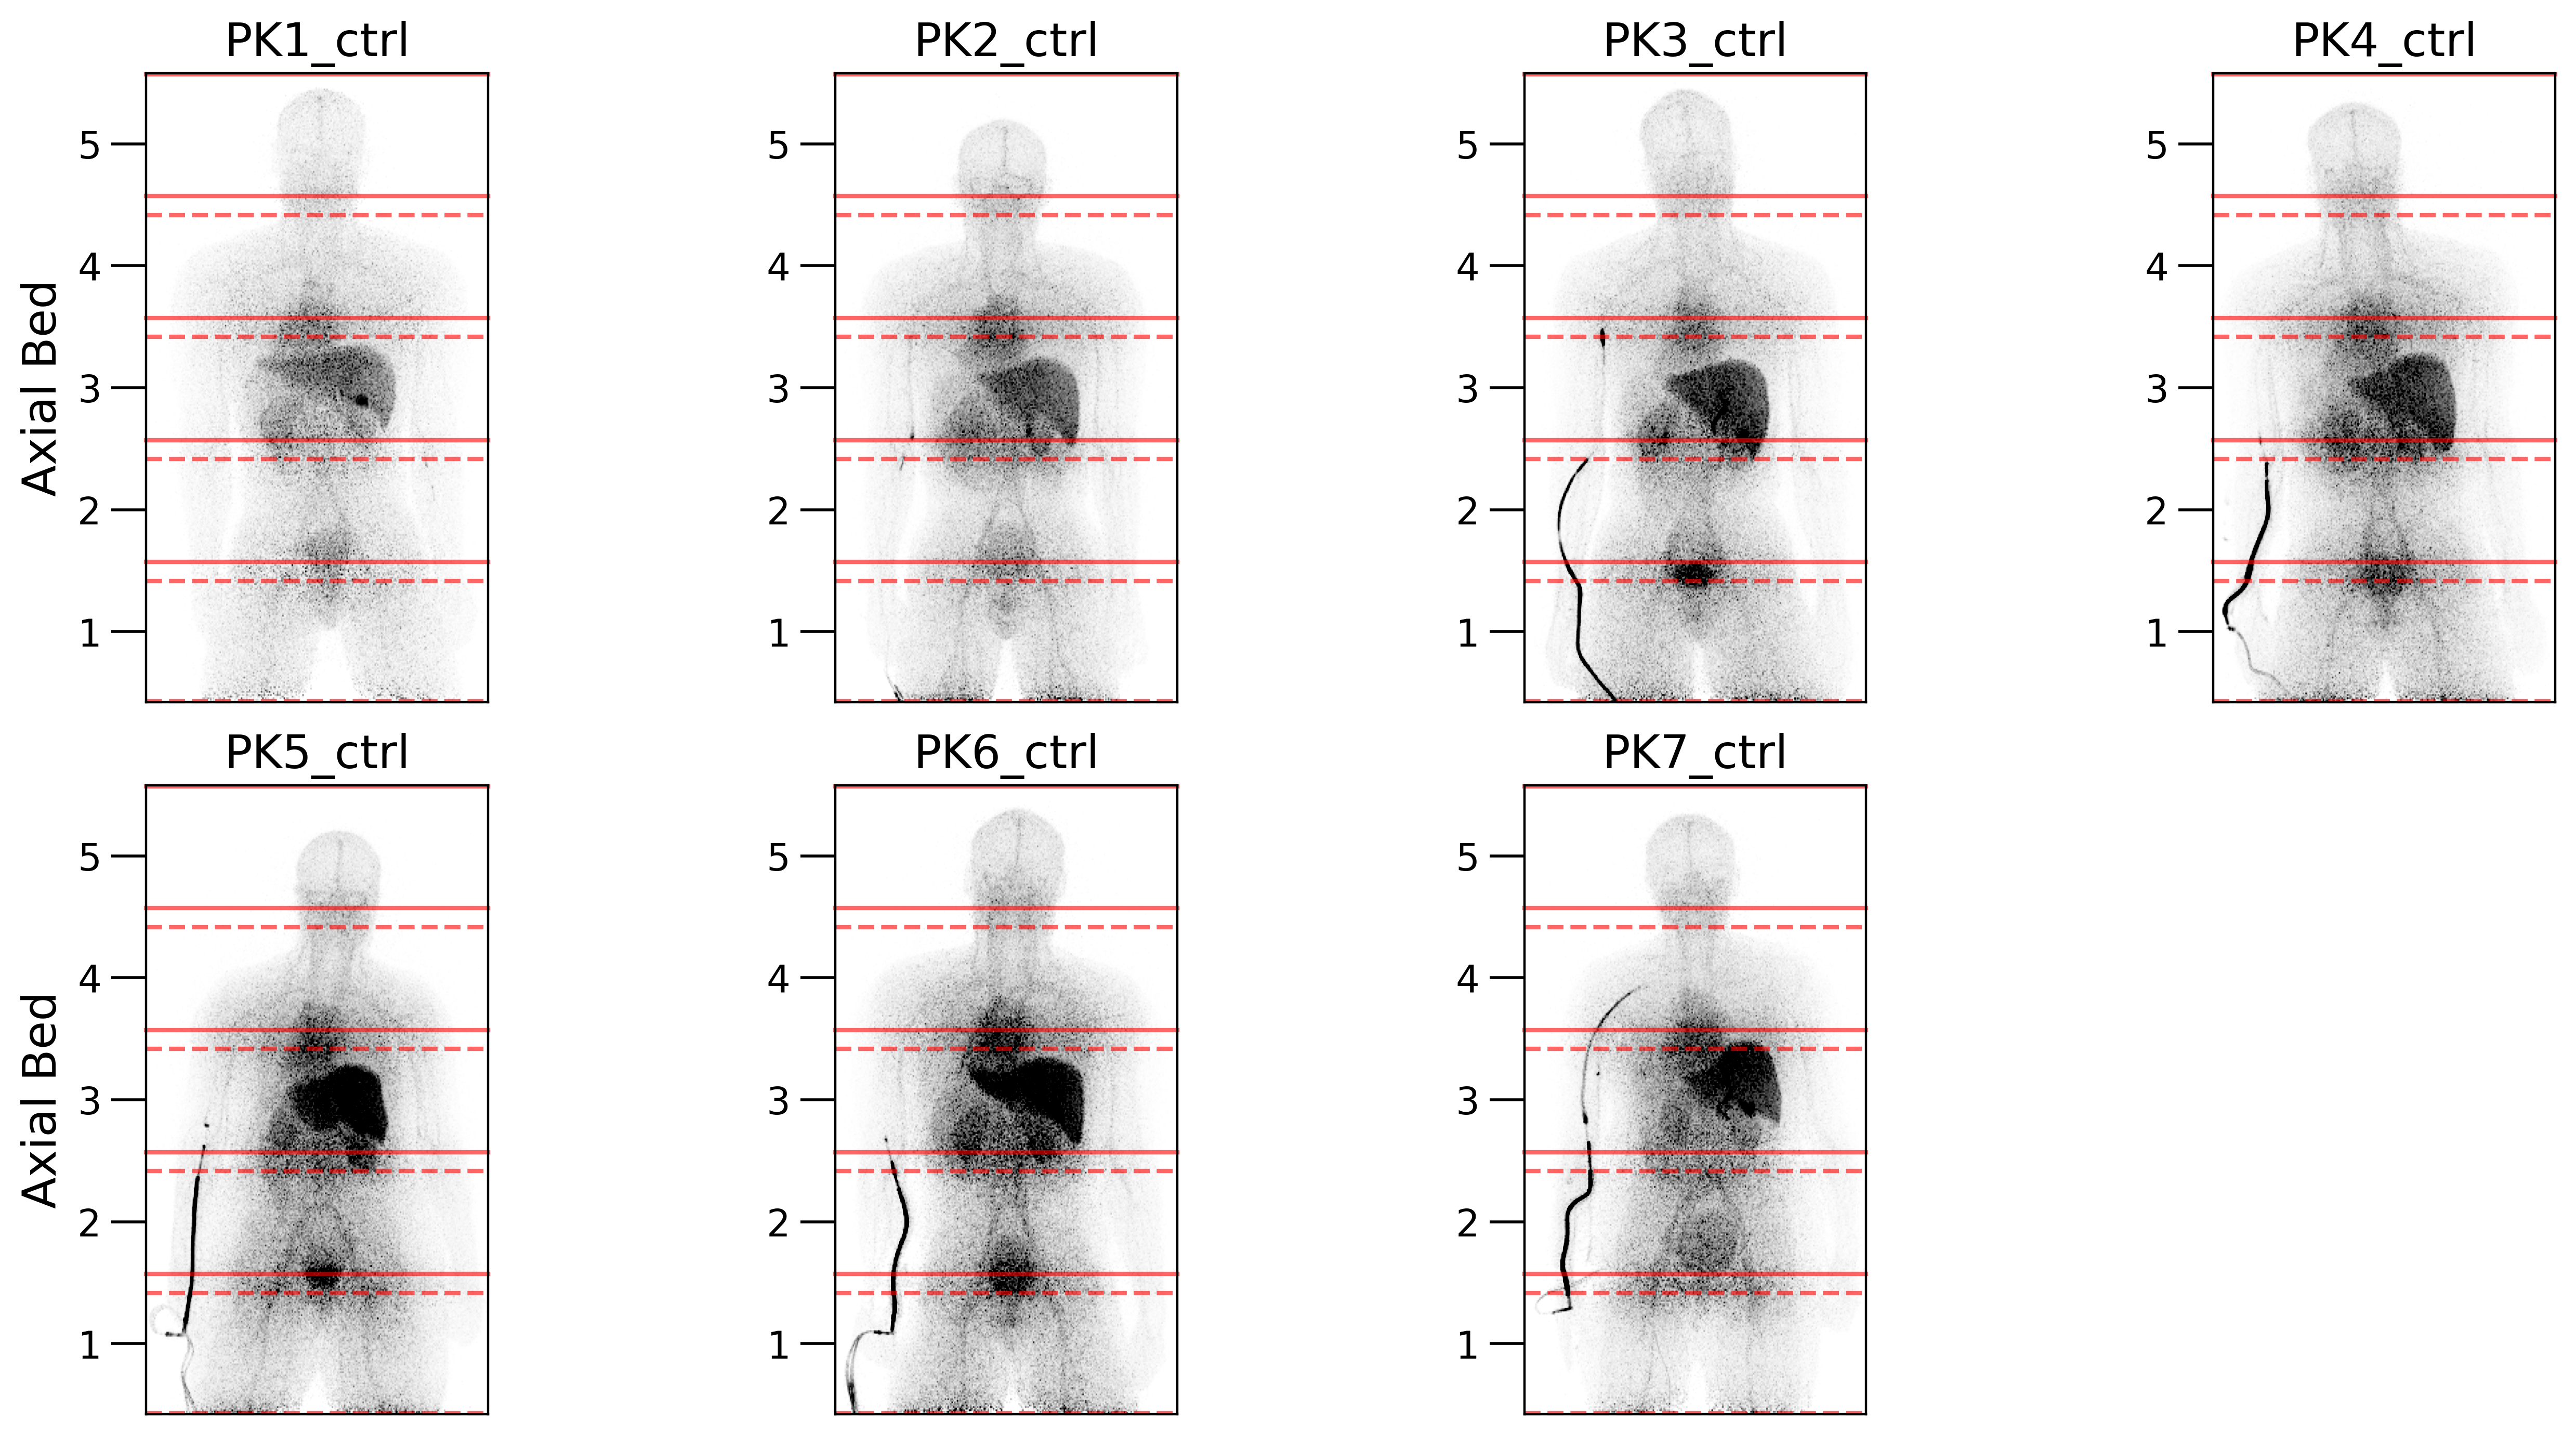
\includegraphics[scale=0.5,angle=0]{3_Results/3_1_DWB_Optimization/figures/3_1_MIPS_ctrl.png}
\caption{MIP projections of 7 volunteer control DWB scans with overlay of axial bed start and end location.} 
%TODO: Add over-scan in the CBM D-WB protocols. 
\label{fig3_1:ctrl_mips}
\end{figure}
%
\begin{figure} [ht!]
\centering
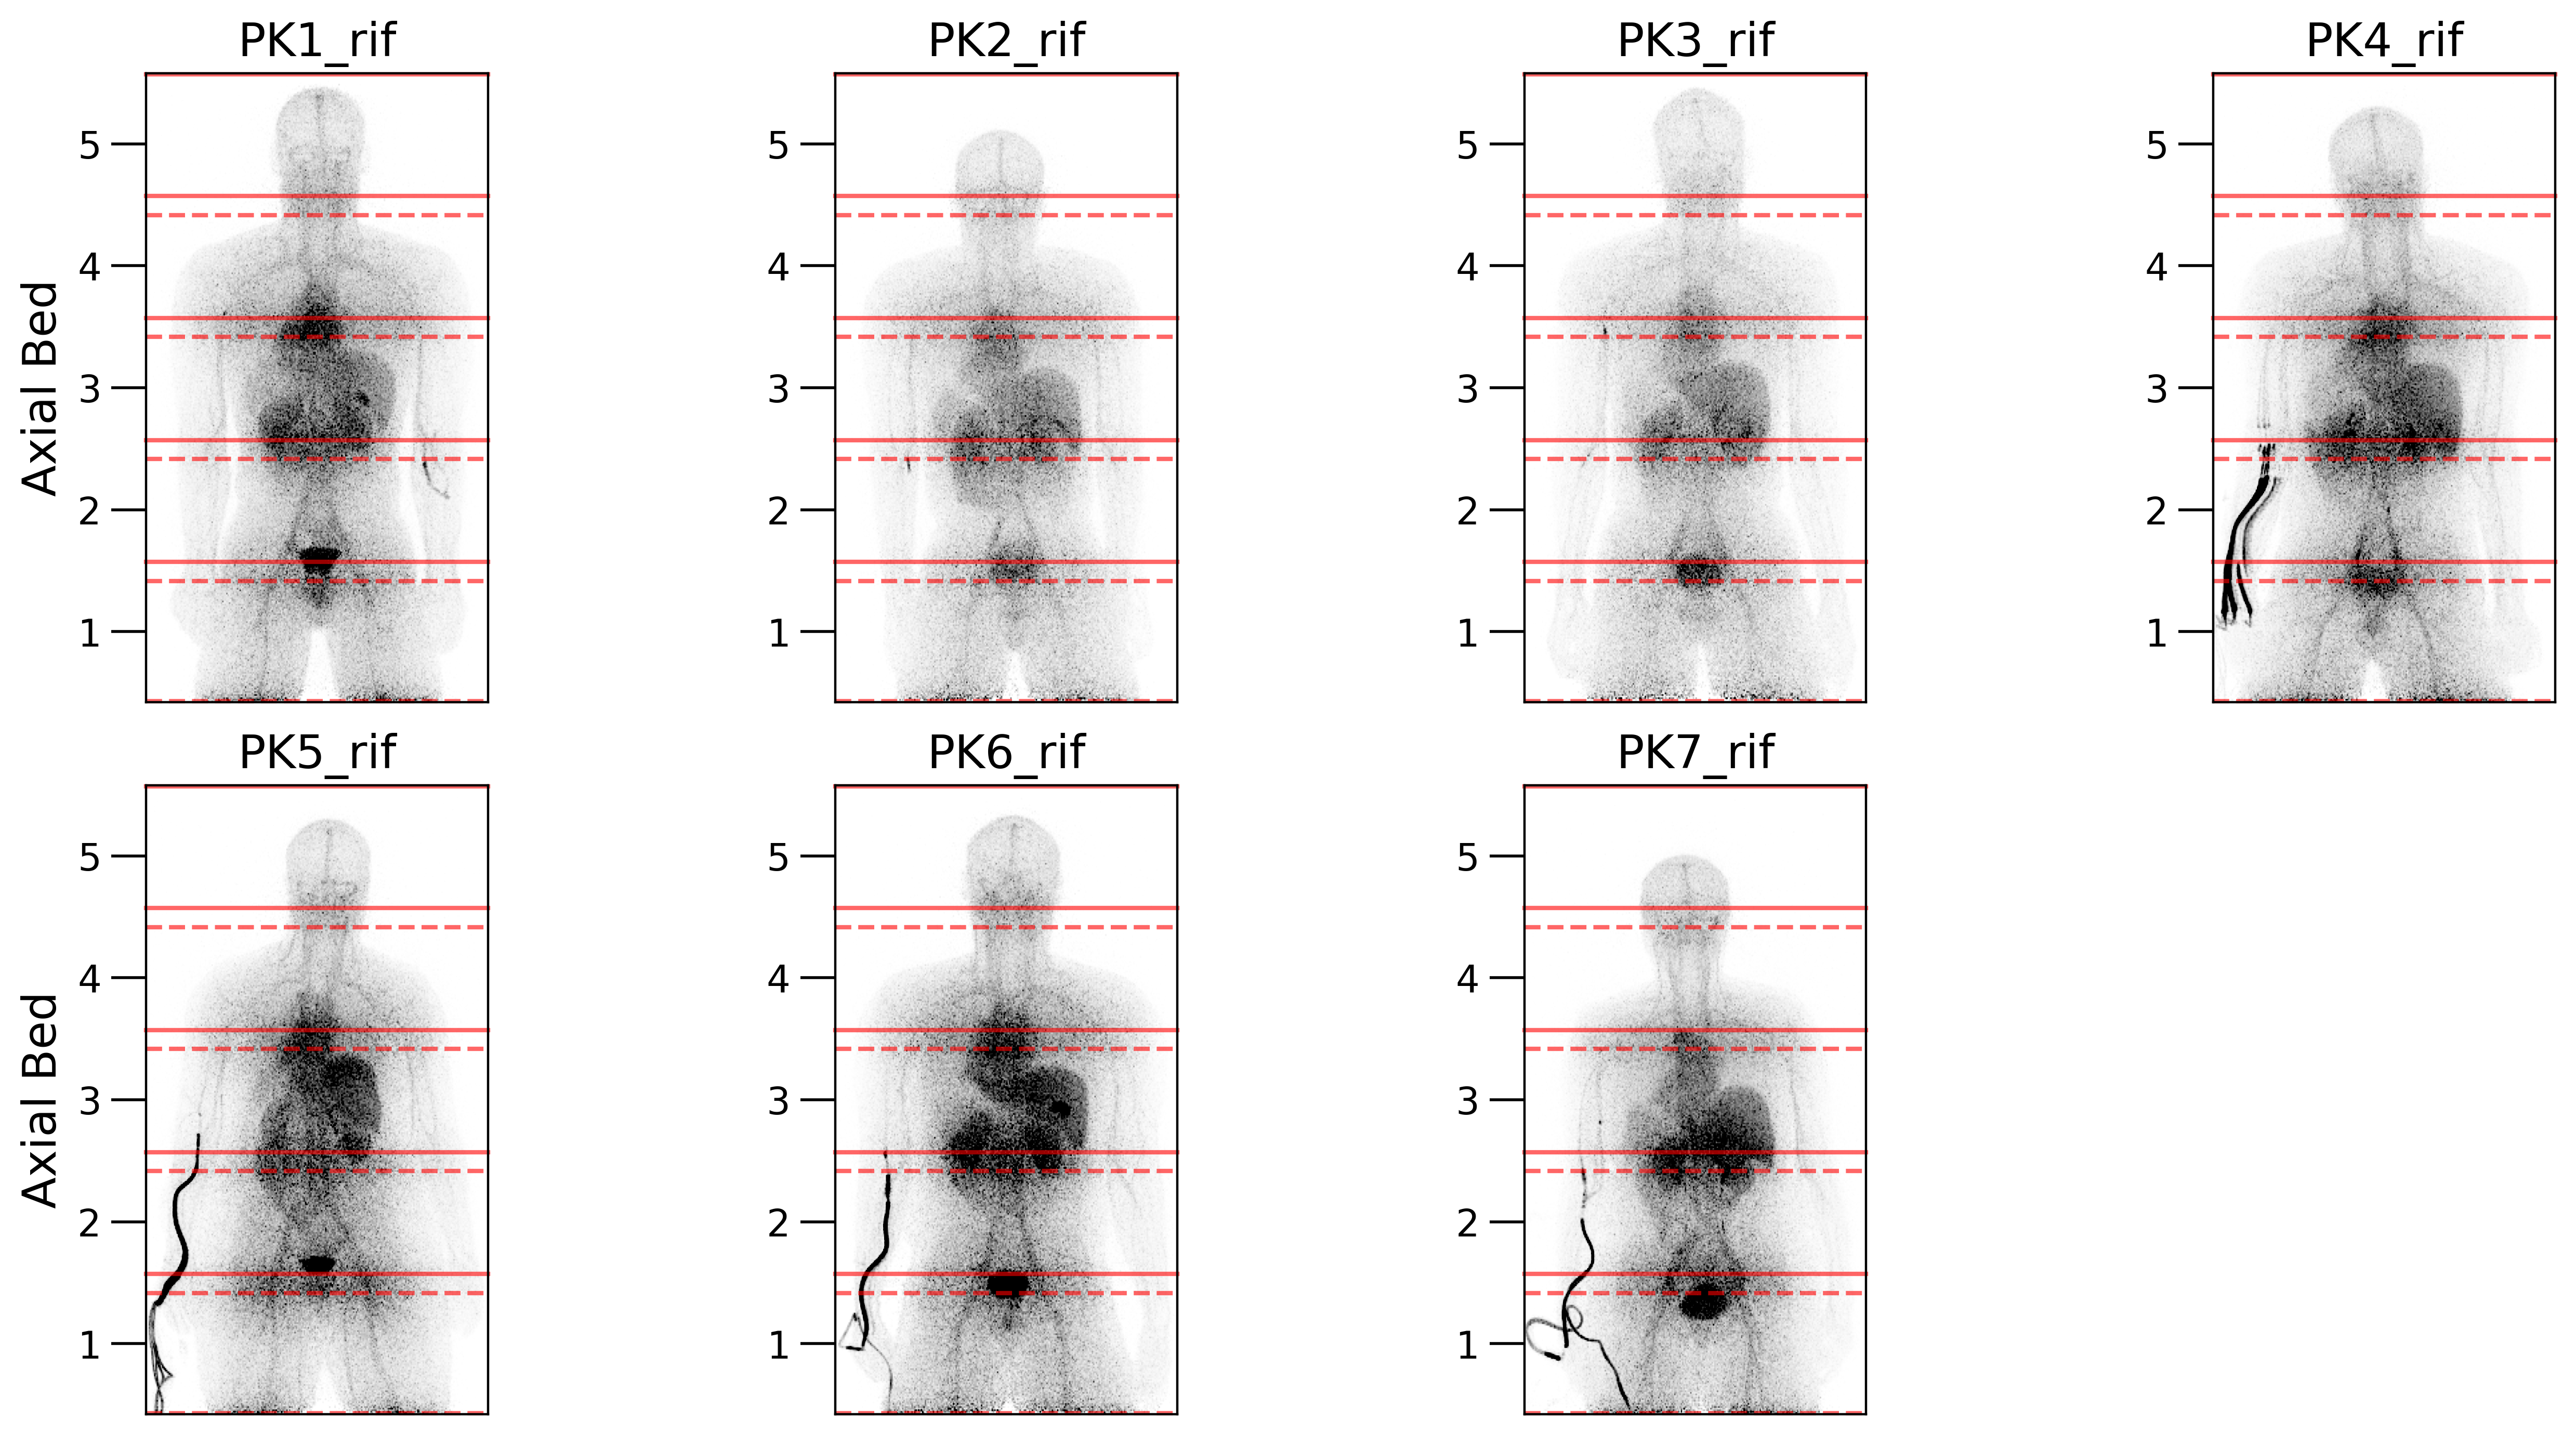
\includegraphics[scale=0.5,angle=0]{3_Results/3_1_DWB_Optimization/figures/3_1_MIPS_rif.png}
\caption{MIP projections of 7 volunteer rif DWB scans with overlay of axial bed start and end location.} 
%TODO: Add over-scan in the CBM D-WB protocols. 
\label{fig3_1:rif_mips}
\end{figure}
%
%
\section{Export and offline reconstruction of IsotoPK DWB data}
Reconstruction of DWB on the Signa PET-MR console is made with certain limitations and does not allow for full and accurate use of the acquired data, with the correct timing information per bed acquisition which is especially important in estimation of parametric maps. \\
To make better use of these datasets, an export and offline processing pipeline was developed as part of this PhD project. The pipeline is based on custom-made python scripts and matlab scripts, that integrate with the GE-PET toolbox. This is a toolbox provided by GE for certain offline reconstruction operations. In this pipeline the Toolbox is used for generation of image corrections. These include normalisation factors, attenuation factors from MRACs, random and scatter corrections as well as dead-time corrections. 

\subsection{Export from Console}
DWB studies are exported from the PET-MR console using a custom export tool provided by GE, that provides the whole study in the following directory structure.  \\
\dirtree{%
.1 {20200110\_e02066\_02-DF-10\ (Date “YYYY-MM-DD”,  StudyID)}.
.2 LST.
.3 LST\_30501\_PET\_CE\_00\_a\_blanc.
.3 LST\_30502\_PET\_Liver.
.3 LST\_30503\_PET\_CE\_01.
.3 LST\_30504\_PET\_CE\_02.
.3 LST\_30505\_PET\_CE\_03.
.3 $\dots$.
.2 MRAC.
.3 WATER\_1\_PET\_CE\_00\_a\_blanc.
.3 WATER\_1\_PET\_Liver.
.3 WATER\_1\_PET\_PET\_CE\_03.
.3 $\dots$.
}

Those are then processed using the custom-made pipeline as follows:
\begin{itemize}
    \item \textbf{Step1: Verify Injection Time} \\
    Before organising the DWB data, it is important to verify the injection time point, to which all the DWB will be decay corrected to. 
    In this pipeline we verify the injection time by inspecting the total prompt to time curve from the list-mode dataset of the single-bed dynamic phase, as shown in figure. 
    \item \textbf{Step2: DWB data sorting} \\
    The data are re-sorted to single directories per WB sweep, where each directory includes the list-mode data of sweep's five bed positions and their corresponding MRACs if acquired. Subsequently, for sweeps with no acquired MRAC, the MRACs of previous sweeps are copied in these directories.
    At this step all the timing information from the headers of the PET list and MRAC files are extracted and saved in a database. 
    \item \textbf{Step3: GE-PET Toolbox processing } \\
    The data in each sweep's directory are unlisted and reconstructed with the GE-PET Toolbox as individual static acquisitions. This process generates the required corrections for reconstruction. Similar processing is applied for the single-bed dynamic phase, which is reconstructed by the toolbox as a dynamic study.
    \item \textbf{Step4: Conversion to CASToR datafiles} \\
    The list-mode raw data and the generated corrections are used to make CASToR list-mode datafiles as well as normalization files for each bed position of the acquisition and for all dynamic frames of the single-bed dynamic phase. 
    The time-tags of each list-mode file are modified accordingly, to the injection time point reference, using the database information build earlier. 
\end{itemize}

\begin{table}[]
\begin{tabular}{lrlrrrrrlr}
\toprule
{Index} &  Bed Instance &  List\ Frame\ Time &  Frame\ Duration & MRAC Number &  MRAC\_AC &  FrameStartTime \\
\midrule
5  &         1 &  152358.301552 &            270 &           18 &          True &         -93.200 \\
6  &         1 &  152854.357026 &             20 &           12 &          False &         202.855 \\
7  &         2 &  152919.427076 &             20 &           13 &          False &         227.925 \\
8  &         3 &  152944.578076 &             20 &           14 &          False &         253.076 \\
9  &         4 &  153009.716076 &             20 &           15 &          False &         278.214 \\
10 &         5 &  153034.852076 &             20 &           16 &          False &         303.350 \\
11 &         1 &  153121.372932 &             20 &           12 &          False &         349.871 \\
12 &         2 &  153146.440050 &             20 &           13 &          False &         374.938 \\
13 &         3 &  153211.581050 &             20 &           14 &          False &         400.079 \\
14 &         4 &  153236.720050 &             20 &           15 &          False &         425.218 \\
\bottomrule
\end{tabular}
\end{table}

The 14 studies shown in figures~\ref{fig3_1:rif_mips} and ~\ref{fig3_1:ctrl_mips} were processed with our pipe-line to enable offline reconstruction and to extract timing information. Using the timing information we were able to estimate the delay times (time gaps) of the DWB protocol used in practice. These are shown in the form of box-plots for $dl_{bed}$ in figure~\ref{fig3_1:BoxPlots_beds} and for $dl_{Sweep}$ in figure~\ref{fig3_1:BoxPlots_sweeps}.
%The average intra-bed delay over the 17 DWB examinations was 7.17 s and the average delay between sweeps was 31 s.
It is noticeable that with experience in running this protocol over time, the delays between sweeps were reduced considerably for the most recent examinations compared to the first. For the 3 more recent subject examinations the average intra-bed delay time $dl_{bed}$ was 5.69 s (95\%CI: 5.63,5.75) and the average delay time between sweeps $dl_{Sweep}$ was 26.17 s (95\%CI: 26.13, 26.22).
These values are close to the one considered in the design of the protocol, but can vary considerably between sweeps of an examination and between examinations.\\
%
%
\begin{figure} [ht!]
\centering
\includegraphics[scale=0.5,angle=0]{3_Results/3_1_DWB_Optimization/figures/3_1_BoxPlots_DTBeds.png}
\caption{Box plots of intra-bed delays $dl_{bed}$ of the IsotoPK DWB protocol used in practice.} 
%TODO: Add over-scan in the CBM D-WB protocols. 
\label{fig3_1:BoxPlots_beds}
\end{figure}
%
\begin{figure} [ht!]
\centering
\includegraphics[scale=0.5,angle=0]{3_Results/3_1_DWB_Optimization/figures/3_1_BoxPlots_DTSweeps.png}
\caption{Box plots of delay between WB Sweeps $dl_{Sweep}$ of the IsotoPK DWB protocol used in practice.}
%TODO: Add over-scan in the CBM D-WB protocols. 
\label{fig3_1:BoxPlots_sweeps}
\end{figure}
%
%
\section{Optimization of DWB acquisition protocol on the Signa PET-MR}
A large fraction of the acquisition delays in DWB protocols are attributed to system processes that are lunched automatically between WB sweeps, such as reconstruction processes and transfer or raw data files. More acquisition time could be gained if those are avoided and delays are decreased. Furthermore the hard-set bed positions do not always allow for optimum use of the effective A-FOV in each examination, as seen for example in examination PK2 in figures~\ref{fig3_1:ctrl_mips}~and~\ref{fig3_1:rif_mips}. In some cases a fewer number of bed positions might be adequate and preferable as it would lead to substantial increase of sampling frequency per bed. \\
Because of these limitations, part of this PhD project was allocated in creating e a fully automated DWB protocol on the Signa PET-MR. The main requirement for the envisioned protocol was to allow for continuous capture of PET data in a single list-mode file for the whole DWB acquisition and for all beds. Then the data could be split to individual bed positions and reconstructed after the acquisition is completed. Using such an acquisition strategy the delays between bed positions and WB sweeps can be reduced to the time taken by the physical motion of the scanner table alone. \\

The PhD schedule included a four week industrial secondment with GE healthcare, for the purpose of exploring tools that could enable the automation of DWB protocols. Three weeks of this secondment were spend at factory facilities of GE healthcare (Waukesha, Wisconsin, USA), where I was given the opportunity the gain insights on the operations of the Signa PET-MR scanner. There with help of the team I was able to exploit in-build factory tools of the Signa PET-MR for the purposes of DWB automation. The two key tools were: 
\begin{itemize}
    \item\textbf{Table Emulation}
    This tool allows for disassociation of the table position between the MR and PET system. It is the key tool that allows for the PET system to acquire continuously, while the MR system commands table motion. The disadvantage of this option is that once table emulation is enabled MR acquisitions cannot be performed.
    \item\textbf{Table Motion}
    This tool commands the MR system to execute movements of the scanner bed. It is a command line tool that requires an input a target bed location and speed before executing the move. 
\end{itemize}
% 
The automated DWB protocol was implemented as a Python class, as the python programming language is available on the PET-MR console and allowed for easy integration of the system tools with user defined routines, all under a common system clock for accurate timing of bed movements and registration of events.\\
The protocol was named "Auto-IsotoPK", but despite its name is a generic DWB protocol that is not limited to the IsotoPK pharmacokinetic study. It allows for an optional single-bed dynamic phase to be acquired before starting the DWB acquisition which can be made for any number of bed positions, customised and defined for each examination on an initial MR scout. A table with the required acquisition times per bed index and WB sweep number is required as input, such as the example table for 3 bed positions and 10 WB sweeps.
Because MR acquisitions cannot be performed after \textit{Table Emulation} is enabled, all bed position MRACs must be acquired prior to the PET examination and used for all WB sweeps of the study.

\begin{table}[ht!]
\centering
\label{tab:TimmingTable}
\caption{Example Timing Table, used as input for the fully automated DWB protocol.}
\begin{tabular}{|l|l|l|l|}
\toprule
\textbf{} & \multicolumn{3}{c|}{Durations(s)} \\ 
\textbf{Sweep} & \textbf{Bed-1} & \textbf{Bed-2} & \textbf{Bed-3} \\
\midrule
1     & 10    & 10   & 10    \\
2     & 10    & 10                        & 10    \\
3     & 10    & 10                        & 10    \\
4     & 20    & 20                        & 20    \\
5     & 20    & 20                        & 20    \\
6     & 20    & 20                        & 20    \\
7     & 20    & 20                        & 20    \\
8     & 20    & 20                        & 20    \\
9     & 30    & 30                        & 30    \\
10    & 30    & 30                        & 30    \\
11    & 30    & 30                        & 30    \\
12    & 30    & 30                        & 30    \\
13    & 30    & 30                        & 30    \\
14    & 45    & 45                        & 45    \\
15    & 45    & 45                        & 45    \\
\multicolumn{4}{|l|}{$\dots$} \\
\bottomrule
\end{tabular}
\end{table}

A short \gls{sop} for the use of the protocol is given in the following steps:

\begin{enumerate}
    \item Load "IsotoPK\_Commander" python class and create new object on a terminal in the PET-MR console. 
    \item Perform scout of subject, plan the desired bed positions for PET acquisition and perform MRAC acquisition. 
    \item Capture the position of the planned PET bed positions.
    \item Load the "Timing Table" with the frame duration per bed positions and sweep number.
    \item If a dynamic phase is required, plan the acquisition and acquire an MRAC for this position. 
    \item Enable table emulation. 
    \item Initiate a one hour long PET acquisition and once acquisition is ongoing perform injection of the subject. 
    \item After adequate time has passed for the single-bed dynamic phase start the automated DWB procedure. 
    \item Once the acquisition has been completed, disable table emulation. 
\end{enumerate}

After the procedure is completed, the whole study is saved in the system as a single-bed dynamic acquisition. The precise timing information of the acquired bed positions are saved in a log file, to be used for the post-processing procedure. 

\subsection{Auto-IsotoPK: Non-Human Primate Study}
After initial tests using phantoms, the protocol was tested on an actual DWB study. A macaque was scanned under full sedation with a novel $^{18}$F-Crizotinib tracer, designed to be used with \gls{nsclc}. A DWB study was required to examine crossing of the blood-brain barrier and study uptake/excretion from other organs. The macaque was injected with 185 \si{\mega \becquerel} of the novel tracer. An initial dynamic phase was requested, centred over the brain for a duration of 90 s, followed by a DWB study of 3 bed positions. The study was planned for an approximate total duration of one hour. A total of 28 WB sweeps and frames per bed were fitted in the study, with the framing of 3$\times$10~\si{\s}, 5$\times$20~\si{\s}, 5$\times$30~\si{\s}, 5$\times$45~\si{\s}, 10$\times$60~\si{\s}. 
Acquisition of the required MRACs was performed prior to injection, at the planned bed positions shown in figure~\ref{fig3_1:Macaque_MRI}. In this acquisition only the body coils of the PET-MR system were used, designed for use with the human body size and load, which resulted in sub-optimal MR quality for automated estimation of attenuation maps. Attenuation maps had to be created manually in post-processing of the data to adequately correct the PET reconstruction for attenuation.  

\begin{figure} [ht!]
\centering
\includegraphics[scale=0.5,angle=0]{3_Results/3_1_DWB_Optimization/figures/3_1_Macaque_MRI.pdf}
\caption{MRAC acquisitions of NHP study showing the planned bed positions of the two acquisition phases.}
\label{fig3_1:Macaque_MRI}
\end{figure}

Following the MRAC acquisitions and after the automated acquisition protocol, the study started with the injection of the NHP subject followed by an hour of PET imaging. 
The complete study dataset was recorded in a single list-mode file, of which the head curve (curve of prompts rate with time) can be seen in figure~\ref{fig3_1:Macaque_Head_Curve}. By overlaying the recorded timing information over this curve, the two phases of the acquisition (SBD and DWB) as well as the three bed position of the DWB acquisition can be distinguished. The initial 260 second of the recorded list-data's head curve with the overlaid phases and bed positions are shown in figure~\ref{fig3_1:Macaque_Head_Curve_Phases}. 

\begin{figure} [ht!]
\centering
\includegraphics[scale=0.45,angle=0]{3_Results/3_1_DWB_Optimization/figures/3_1_Macaque_Head_Curve.pdf}
\caption{Head curve (prompts rate against time) of the acquired NHP study DWB data in a single list-mode file using the optimised protocol.}
\label{fig3_1:Macaque_Head_Curve}
\end{figure}

\begin{figure} [ht!]
\centering
\includegraphics[scale=0.45,angle=0]{3_Results/3_1_DWB_Optimization/figures/3_1_Macaque_Head_curve_Phases.pdf}
\caption{Head curve (prompts rate against time) of the acquired NHP study showing the SBD and DWB phases of the acquisition and the three DWB bed positions.}
\label{fig3_1:Macaque_Head_Curve_Phases}
\end{figure}
%
Using the timing information recorded by in the log file, the data were split into four individual bed position datasets and were processed with the GE-PET toolbox individually as single bed dynamic studies. The list-mode data along with the generated corrections were then exported into the CASToR data-file format for subsequent reconstruction tests. A \gls{mip} view of 3D reconstructions (averaged across all dynamic frames) is shown in figure~\ref{fig3_1:Macaque_PET}. \\
An image derived input function was estimated from the PET data using the right carotid VOI, which was visible on both phases of the acquisition, and the left ventricle. Both VOIs provided similar blood activity values in the DWB phase and were averaged to produce the final IDIF.
%
\begin{figure} [ht!]
\centering
\includegraphics[scale=0.45,angle=0]{3_Results/3_1_DWB_Optimization/figures/3_1_Macaque_PET.pdf}
\caption{MIP views of the NHP study's reconstructed PET images, for the two phases of the acquisition.}
\label{fig3_1:Macaque_PET}
\end{figure}
%
%
\begin{figure} [ht!]
\centering
\includegraphics[scale=0.45,angle=0]{3_Results/3_1_DWB_Optimization/figures/3_1_NHP_InputFunction.pdf}
\caption{NHP study's image derived input function using information from multiple bed positions.}
\label{fig3_1:Macaque_PET}
\end{figure}
%
Using the log timing information an estimation of the delays (time gaps) for this single NHP study using the automated acquisition protocol was made. The results showed an average intra-bed delay time $dl_{bed}$ of 3.77 s (95\%CI: 3.62,3.91) and an average delay time between sweeps $dl_{Sweep}$ of 4.6 s (95\%CI: 4.53, 4.67).

\subsection{Auto-IsotoPK: Continuous Bed Motion on the Signa PET-MR}
The flexibility offered by the use of the automated protocol and the dedicated \"Table Motion\" tool allowed for testing the proof of concept of CBM on the Signa PET-MR scanner. Although this acquisition mode is not supported by the system, we emulated the acquisition of a single whole-body sweep by commanding a table movement at a speed of \SI{5}{\milli\metre\per\second}. The duration of the total sweep, that covered the three bed positions that were acquired in the previous DWB study and included an 50\% overscan, was ...